\chapter{提案手法} % 一般の人がわかるレベルのアルゴリズム解説
\label{chap:approach}

本章では、以上で述べた課題に対して本研究が提案する手法を述べる。

\section{手法の概要}
本研究が提案する手法は、期待和了巡目という途中局面の静的指数を評価することで、適切な打牌を選択するアルゴリズムである。
与えられた牌姿において、和了形までにかかるツモの回数を和了までの消費巡目と定義する。ここで、麻雀においてはどのような牌をツモってくるかは確率的にしかわからず、確定的な情報ではない。したがって、和了までの消費巡目は同じ牌姿であったとしてもそれぞれの場合において異なる可能性がある。そのため、それらを十分な回数行った場合に収束することが期待される平均的な消費巡目を考える。これを、この論文では以下その牌姿における期待和了巡目とする。

% \begin{figure}[h]
%  \centering
%  \includegraphics[keepaspectratio, scale=0.5,bb=0 0 620 439]
%       {img/zu.jpg}
%  \caption{期待和了巡目}
%  \label{zu}
% \end{figure}

\section{期待和了巡目の算出}

% \subsection{有効牌のブロック}

期待和了巡目を求めるためには、まず最初に有効牌のブロックを定義する。有効牌のブロックとは、同じブロック内の有効牌のいずれかを牌姿に加えることで、シャンテン数が1つ少なくなり、2つ以上加えてもシャンテン数がそれ以上下がらないような集合とする。また、本論文において有効牌とは直接シャンテン数を下げる効果を持つ牌のこととし、受け入れが広くなるような二次有効牌については考慮しないことに注意いただきたい。具体例を図\ref{block}に示す。この牌姿の場合、有効牌のブロックはマンズの69、ピンズの46、ソーズの7の3つとなる。この牌姿の場合はシャンテン数は2シャンテンであるが、マンズの6を手牌に加えることでシャンテン数が1シャンテンになる。したがってこの場合マンズの6は有効牌であるが、この1シャンテンの状態でさらにマンズの9を手牌に加えてもシャンテン数は1のままである。そのため、マンズの6と9は同じ有効牌のブロックに属することがわかる。ピンズの46、ソーズの7についても同様である。

\begin{figure}[h]
 \centering
 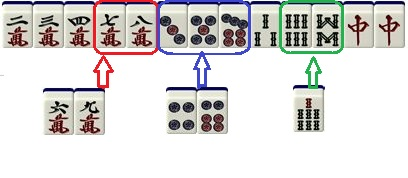
\includegraphics[keepaspectratio, scale=1,bb=0 0 320 194]
      {img/block.jpg}
 \caption{有効牌のブロック}
 \label{block}
\end{figure}

% \subsection{ブロック同士が独立}
1つの有効牌のブロックによって、シャンテン数が1さがるような平均消費巡目は、そのブロックの有効牌を一回のツモでツモる確率をpとすると、

\begin{equation}
\label{kitai1}
\Large \lim _{k\rightarrow \infty }\sum { kp(1-p)^(k-1)} = \displaystyle \frac{1}{p}
\end{equation}

と表される。したがって、平均の考え方を使うことでブロック同士が独立である場合は、これを複数のブロックにも拡張できる。

% \subsection{ブロック同士が重複}
また、ブロック同士が重複している場合においては、複雑な計算が必要となる。したがって本研究では、重複したブロックに存在する有効牌についてはどちらか片方に入れて計算するようにする。


% 【この計算手法についてはもう少し書きます】

% \subsection{ブロックがオーバーしている場合}








\section{想定されるメリット}
この節では、以上に提案した手法を関連研究の事例を交えて、優位性があると期待される部分について述べる。
まず最初に本手法と同じく与えられた牌姿に対して途中局面の静的指数を評価することで妥当である牌姿を選択するアルゴリズムを挙げる。これらは、モンテカルロ法などのシミュレーションをプレイアウトまで行わないものである。また、関連研究としては本手法と同じく期待和了巡目と近い考え方を用いた例を述べる。しかし、この例では期待和了巡目の算出にモンテカルロ法によるシミュレーションを使っており、静的な評価方法ではない。また、期待和了巡目の算出方法も、ツモったあとに切らないという考え方を使っており、正確な評価ではない点がある。


\subsection{シャンテン数を下げるアルゴリズムとの比較}
麻雀において、特定の和了までに必要な牌の数がシャンテン数であるため、与えられた牌姿においてのシャンテン数を把握することは和了のしやすさを評価することにつながる。これは最も基本的な方法であるため、あらゆる麻雀AIの研究で基礎として行われている。三木ら\ref{mikiUCT}は、UCTアルゴリズムの評価を行う際に、グリーディングプレイヤーとして、シャンテン数を下げるように打つプレイヤーを用いている。このグリーディングプレイヤーでは、与えられた牌姿の中で打つことのできる全ての牌に対して、打った後のシャンテン数を調べる。その後、元の牌姿とそれらのシャンテン数をそれぞれ比較し、シャンテン数が小さくなるような手を選択するアルゴリズムである。シャンテン数が同じように小さくなる手が複数あった場合には、ランダムでその中から選んだものを選択するようになっている。具体例を図\ref{yuko}に示す。

\begin{figure}[h]
 \centering
 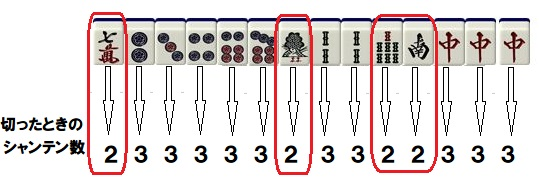
\includegraphics[keepaspectratio, scale=1,bb=0 0 539 194]
      {img/syanten.jpg}
 \caption{シャンテン数下げるように打つアルゴリズム}
 \label{syanten}
\end{figure}

この手法の問題点は、シャンテン数を下げる牌の中が複数あるときにランダムで打牌を選択しているところにある。一般にある牌姿からシャンテン数を下げる牌は複数あることがほとんどであり、ここでランダムな要素を入れてしまうと、その中での優劣を比較できない。シャンテン数を下げる牌の中でも牌の優劣を決めるための方法として、有効牌の数を比較する手法があげられる。これについて次節で解説する。


\subsection{有効牌の数を数えるアルゴリズムとの比較}
有効牌とは、シャンテン数を下げる牌のことである。具体例を図\ref{yuko}に示す。

\begin{figure}[h]
 \centering
 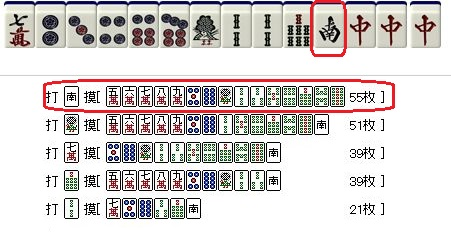
\includegraphics[keepaspectratio, scale=1,bb=0 0 320 239]
      {img/yuko.jpg}
 \caption{有効牌が多くなるように打つアルゴリズム}
 \label{yuko}
\end{figure}

この牌姿では、マンズの7、ソーズの1、7、字牌の南のどれを切ってもシャンテン数は下がるが、有効牌の数は異なる。有効牌の数を比較すると、それぞれ39、51、39、55となっていて、55である字牌の南を切ることになる。このアルゴリズムは、佐藤ら\cite{zentsu}の研究で詳しく行われている。この方法の問題点は、同じ有効牌の数であっても、ブロックの構成要素の違いを理由に和了率が異なるという点が挙げられる。また、佐藤らの研究では、目先の有効牌だけを比較するのではなく、再帰的に次の展開の有効牌も比較しているが、最終的には末端の有効牌を比較しているためそれまでの関連性が排除されている。したがって和了にたどり着くまでのシャンテン数が大きければ大きいほど実際の和了率を挙げる選択とかけ離れる問題がある。


\subsection{擬似的に期待和了巡目をモンテカルロ法で行った研究との比較}

水上ら\cite{bakuuti}の研究の前衛である、「麻雀を打つ機械」\cite{nmizu}の牌効率のアルゴリズムでは、モンテカルロ木探索を用いている。
そのアルゴリズムの概要を図\ref{fig:monte1}に示す。
ツモを入れた状態で14枚の牌姿から、それぞれ切ることのできる牌を切った場合を一つのノードとする。この場合深さ1の14つのノードができることになる。
この後、それぞれのノードの状態から、ツモることの可能な牌をランダムにツモっていくシミュレーションを行う。この場合ツモる事のできる牌とは、場や自分の手牌に情報として見えている牌をゲーム開始時に存在する麻雀牌セットの中から抜いたものである。通常麻雀のルールでは、牌をツモることで次に捨てるという動作が発生するが、ここではそれを行わない。これをしないことで、探索空間が膨大に膨れ上がるの防ぐ効果があり、特定のシミュレーション時に最速で上がるための手順を特定することが可能となる。ツモを連続で行っていき、それまで手牌に残っていた牌の組み合わせで和了することができる場合となるまでシミュレーションを行い、上がった場合にプレイアウトとなる。このシミュレーションを各ノードでそれぞれ十分な回数行い、プレイアウト発生するまでのツモった回数の平均とり評価値とする。最後に、各ノードの評価値を比較し、最もこの値が少なかったノードが最適な打牌と考え選択することになる。プレイアウトまでにツモった回数の平均が少なければ少ないほど、より早く和了できることが期待されるからである。

\begin{figure}[h]
 \centering
 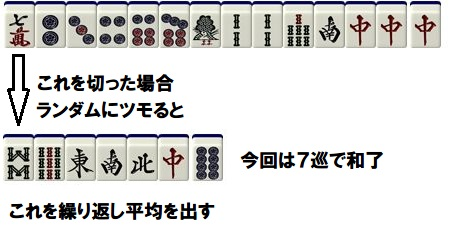
\includegraphics[keepaspectratio, scale=1,bb=0 0 300 200]
      {img/monte1.jpg}
 \caption{モンテカルロ法で期待和了巡目を求めるアルゴリズム}
 \label{monte2}
\end{figure}


% \section{想定されるデメリット}

% \subsection{変化を考慮した期待和了巡目の計算}

% 国士氏の研究により、ある手牌における聴牌までの平均消費順目は、それぞれの変化での平均消費巡目のそれぞれの変化する確率での単純な平均で与えられることがわかっている。[3]すなわち、図\ref{kokusi}に示すように、元の成功率がp、手変わりする確率がq,r、手変わり後の成功率がQ,Rならば、

% その手の向聴が進むまでの平均消費巡目は

% \begin{equation}
% \label{kitai1}
% \Large \displaystyle \frac {p\frac{1}{p} + q\frac{1}{Q} + r\frac{1}{R}}{p+q+r}
% \end{equation}

% と表される。


% 変化の牌姿



% この式\ref{kitai1}は、他プレイヤによって捨てられた牌を使ったシャンテン数現象パターン、すなわち鳴きを考慮していない。したがって面前聴牌のみを考えた式ということになる。しかし、1人麻雀においては相手プレイヤを考慮しないため、1人麻雀における聴牌率は4人麻雀における面前聴牌確率と一致し、この式によって求まる。鳴きによって聴牌する有効牌については、全て面前ツモで聴牌する有効牌の一部であり、制限によって鳴くことが出来ない有効牌も多く存在する。例えば、以下のような牌姿の場合である。


% ヘッドレスイーシャンテンの牌姿を見て解説
% 図


% また、面前聴牌と鳴きによる聴牌の違いについては、麻雀の役の性質上、和了することができなくなる制約や、点数が下がるなどの問題がある。したがって、鳴くことによる聴牌が面前聴牌に与える影響は少ないと考えられる。

% ここで、本論文ではこれを和了時までの式に拡張する。

% まず平均の関係から

% \begin{figure}[h]
%  \centering
%  \includegraphics[keepaspectratio, scale=0.1,bb=0 0 4032 3024]
%       {img/math.jpg}
%  \caption{}
%  \label{math}
% \end{figure}

% \begin{equation}
% \label{kitai2}
% \Large \displaystyle \frac {p\frac{1}{p} + q\frac{1}{Q} + r\frac{1}{R}}{p+q+r}
% \end{equation}


% ここで和了期待順目について考える


% 前節と同様に、4人麻雀において聴牌した

% 面前で聴牌するための平均消費順目と鳴きを考慮

% まず、聴牌までの平均順目と聴牌後の和了までの平均順目の合計がすなわち全体の平均消費順目であることを証明する。
% 次に、それを合成した結果の数式がどうなるかを書く。

% 考察の結果このようになる。

% \begin{equation}
% \label{kitai2}
% \Large \displaystyle \frac {p\frac{1}{p} + q\frac{1}{Q} + r\frac{1}{R}}{p+q+r} + 和了期待順目
% \end{equation}
% また、(現在の平均テンパイ巡目)=(次巡の平均テンパイ巡目)+1 であることから、
% 各ノードが手替わり率とテンパイ率を値として持つ深さ1の木構造で記述できる。 
% したがって、同様に、n手先の手替わりまで考えると深さnの木構造で記述することができる。
% nを大きくすることにより、精度の高い和了率を近似することが可能となる。

% \begin{figure}[h]
%  \centering
%  \includegraphics[keepaspectratio, scale=0.1,bb=0 0 4032 3024]
%       {img/pqr.jpg}
%  \caption{}
%  \label{math}
% \end{figure}

% 本研究では、この式(3)をそれぞれの牌姿に当てはめ、その計算結果が高くなるようなノードを探索する。
% これにより、従来の手法では何回も同じ牌姿の変化をシミュレートしなければいけない問題があったが、(3)式の評価によってその多くが削減できる。
% したがって、この方法によって精度が高くなることが期待される。


% \section{和了率の評価によるノードの展開}

% 本研究では、モンテカルロ法の探索空間が大きくなりすぎる問題に対して、特定のノードの牌姿に対する期待和了順目を次の節で説明する数理モデルを使って有望だと思われる手を探索するようにする。
% 1人麻雀において特定の牌姿の期待和了順目を途中で評価できることは、より有望な手を探索できる可能性がつながるため、UCB1などの評価値よりも手の有望さを評価する精度を上げることができると期待される。

% ・期待和了順目の計算式とその証明
% ・ノード構造でできることの解説
% ・ノードをどこまで探索した方がいいかということについて
% →シャンテン数がでかすぎる場合は期待和了順目の精度が落ちること
% ・そのため、シャンテン数のでかすぎる場合についてはシャンテン数が下がる選択(有効牌は数える)
% →てかそれはそもそもそのままシャンテン数が上がる確率で求めているだけでは?
% →シャンテン数が進む場合の平均消費順目を計算しているだけ
% 期待和了巡目としても計算は可能では?実質同じっぽい。ただどこまで変化を入れるか。目先の変化だとびみょい。

% 期待和了巡目もそもそも実質有効牌を数え上げているだけだから(ただし、一巡進んだ後に排除しなければいけない有効牌を覗かないといけない。)
% これをシャンテン数がでかすぎる場合に当てはめても可能といえば可能。
% ただ当然精度が落ちる。が、そもそも有効牌を数え上げて切っているアルゴリズム自体がやってることが同じなので、これをこのまま当てはめれば多分行ける。
% 理論上は可能な気がする。

% \begin{figure}[h]
%  \centering
%  \includegraphics[keepaspectratio, scale=0.5,bb=0 0 304 387]
%       {img/UCB.png}
%  \caption{和了率評価を用いたモンテカルロ木探索}
%  \label{monte2}
% \end{figure}



% \subsection{プレイアウトと平均報酬}

% \begin{figure}[h]
%  \centering
%  \includegraphics[keepaspectratio, scale=0.1,bb=0 0 4032 3024]
%       {img/playout.jpg}
%  \caption{}
%  \label{math}
% \end{figure}

% 普通に展開した場合は平均報酬と期待和了巡目の関連性がないので、そこが問題。
% 単純に期待和了巡目で比較するか、そもそも期待和了巡目を報酬とすることで書き換えていくか。

% \subsection{二向聴以下の牌姿に対してモンテカルロ法を適用する}

% 麻雀において、和了までの手順の中では、シャンテン数が小さい時点での選択が成績に影響を与えやすいことがわかっている\cite{gendai}
% したがって、成績向上のためには和了系に近い部分において戦略を改善することが成績に影響を与えやすい事がわかる。

% また、モンテカルロ法の問題点は、前述したとおり麻雀に適用すると探索空間が大きくなりすぎることが問題であった。しかしこれを和了系に近い部分に適用することで、
% 探索空間を小さく削減することができるため、適用することができるようになる。
% 本研究の手法である与えられた牌姿における和了率の近似式(3)を適用する際にも、シャンテン数が大きすぎる場合については正確に見積もることが難しいため、このような限定的な部分への適用が重要である。

% 本論文では二向聴以上の部分にこのモンテカルロ法を適用することで、従来の問題点を解決する。
